
\noindent\textbf{1. (CRLS 23.1-1)} Seja $e$ uma aresta de custo mínimo em um grafo $G$ com custos nas arestas. É verdade que $e$ pertence a alguma MST de $G$? É verdade que $e$ pertence a toda MST de $G$?\\[6pt]
\textbf{Resposta:} Seja $A$ um subconjunto de arestas de alguma MST $T$, tal que $(u, v) \notin A$. Para escolher uma aresta para ser adicionada em $A$, todas as arestas que atravessam um corte $(S, S-V)$ são consideradas. Como o corte deve respeitar $A$ e a aresta $(u, v)$ tem peso mínimo, ela será escolhida para ser incluída em $A$, o que dá origem a uma nova MST $T'$, onde $A \cup \{(u, v)\} \subseteq T'$.

\textbf{É verdade que $e$ pertence a toda MST de $G$?}
Não é verdade. Se tomarmos uma aresta $(u, v) \in E$ de uma MST $T$ que tenha custo mínimo $k$ e substituirmos por outra $(u, w)$ que não está em $T$ de custo $k = l$, teremos uma nova MST $T'$, ou seja, é o caso onde há empate na escolha da aresta segura para ser incluída na árvore. Portanto, $e$ não pertence a toda MST de $G$.

Na figura \ref{fig:8.1-1}, basta substituirmos a aresta $(b, c)$ pela $(b, d)$ e teremos uma nova MST de mesmo custo mínimo.
\begin{center}
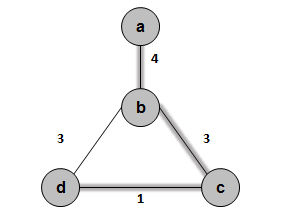
\includegraphics[width=0.4\textwidth]{q8-01.png}
\captionof{figure}{MST com mais de uma aresta de mesmo custo.}
\label{fig:8.1-1}
\end{center}